\section{Análisis comparativo}

\subsection{Comparativa entre el filtro neuronal y el estado del arte}

Resulta relevante comparar los resultados obtenidos con aquellos descritos en la sección \ref{sec:estado_del_arte}. Llamemos al filtro neuronal \emph{FN} y al filtro adaptativo \emph{FA}. A continuación podemos ver la tabla comparativa:

\begin{table}[H]
	\centering
	\begin{tabular}{ |c|c|c|c|c|c|c|c| } 
		\hline
		& TR2 & TR5 & TR6 & TR7 & FN & FA \\ 
		\hline
		PESQ - Ruidosa & 2.33 & 2.22 & 2.22 & 2.52 & 2.20 & 2.20 \\
		PESQ - Filtrada & 2.84 & 2.65 & 2.55 & 3.11 & 2.40 & 2.16 \\
		PESQ - Mejora & 22\%  & 19\% & 14\% & 23\% & 9\% & -2\% \\
		\hline
		STOI - Ruidosa & 0.81 & 0.88 & 0.88 & 0.92 & 0.88 & 0.88 \\
		STOI - Filtrada & 0.87 & 0.91 & 0.88 & 0.95 & 0.87 & 0.90 \\
		STOI - Mejora & 7\% & 3\% & 0\% & 3\% & -1\% & 2\% \\
		\hline
	\end{tabular}
	\caption{Comparación de resultados.}
\end{table}

Los resultados obtenidos para el filtro neuronal \emph{FN} son cercanos a los obtenidos en \emph{TR6}. Ambos trabajos utilizan la misma base de datos \cite{a_scalable_noisy_speech_dataset_and_online_subjective_test_framework}. El mejor desempeño en el trabajo \emph{TR6} radica en el tipo de arquitectura utilizada. La red recurrente que utilizo \emph{TR6} tiene la ventaja de no tener que establecer manualmente parámetros como $J$ y el tamaño de los filtros de las capas convolucionales. Recordemos que el tamaño de los filtros establecen limites en la correlación entre las distintas muestras tanto en tiempo como en frecuencia. Estos hiperparámetros, para el caso de la red recurrente, son optimizados durante el entrenamiento. 

Si bien, las redes recurrentes tienen la ventaja de tener menor cantidad de hiperparámetros, tienen la desventaja de tener un proceso de entrenamiento mas complejo. Es por esto que en el presente trabajo se decidió utilizar arquitecturas mas simples como la convolucional.

Respecto a la diferencia con trabajos como \emph{TR2}, \emph{TR5} y \emph{TR7}, la principal diferencia radica en la base de datos. La base utilizada en la presente tesis, tiene una duración total de 38 horas y 14 tipos de ruidos distintos. Los trabajos \emph{TR2} y \emph{TR7}, utilizaron bases con mas de 100 horas de duración y con mas variedad de ruidos. El trabajo \emph{TR5} si bien utilizo la misma cantidad de ruidos, tilizo técnicas para incrementar hasta las 100 horas de duración total. 

A medida que se aumenta el tamaño de las bases de audios, aumenta la complejidad del entrenamiento. Para procesar 100 horas de señales de audio, aproximadamente se necesita un tiempo similar de entrenamiento con una sola GPU para recorrer al menos 1 vez todo la base. La decisión de utilizar la base de datos \cite{a_scalable_noisy_speech_dataset_and_online_subjective_test_framework} radicó en mantener el entrenamiento lo mas simple posible.

Por último cabe destacar que los trabajos \emph{TR5}, \emph{TR6} y \emph{TR7}, utilizaron el rango [0, 20] dB para mezclar los ruidos. En el presente trabajo y en \emph{TR2}, el rango utilizado fue [-5, 20] dB. Esta diferencia, en el valor medio informado contribuye a un mejor desempeño global ya que, en general, el desempeño de la red disminuye en bajos SNRs. Como ya vimos en la sección anterior, esto se debe a que a bajos SNRs la red aplica mayor supresión de ruido lo cual a su vez genera mayor distorsión y por ende menor calidad e inteligibilidad.

\subsection{Comparativa entre el filtro adaptativo y el neuronal}

En las secciones anteriores pudimos ver el desempeño de cada filtro por separado. Veamos ahora la comparativa utilizando las medidas PESQ y STOI. En la figura \ref{fig:ch8_pesq_comparison_by_snr} podemos ver la medida PESQ - Filtrada, tanto para el filtro adaptativo como para el filtro neuronal, para los distintos niveles de ruidos utilizados.

\begin{figure}[h]
	\centering
	\centerline{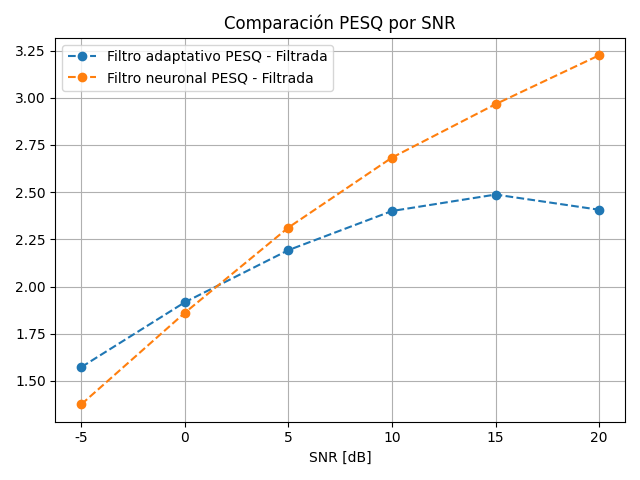
\includegraphics[scale=0.75]{images/ch8/comparison_pesq_by_snr.png}}
	\caption{Comparación PESQ en función de la SNR.}
	\label{fig:ch8_pesq_comparison_by_snr}
\end{figure}

Podemos ver en la figura \ref{fig:ch8_pesq_comparison_by_snr} que a altos niveles de ruido (SNR bajos), el desempeño del filtro adaptativo fue levemente superior, sin embargo aproximadamente a partir de los $\SI{0}{dB}$ el filtro neuronal superó al filtro adaptativo.	

En la figura \ref{fig:ch8_stoi_comparison_by_snr} podemos ver la medida STOI - Filtrada, tanto para el filtro adaptativo como para el filtro neuronal, para los distintos niveles de ruidos utilizados.

\begin{figure}[H]
	\centering
	\centerline{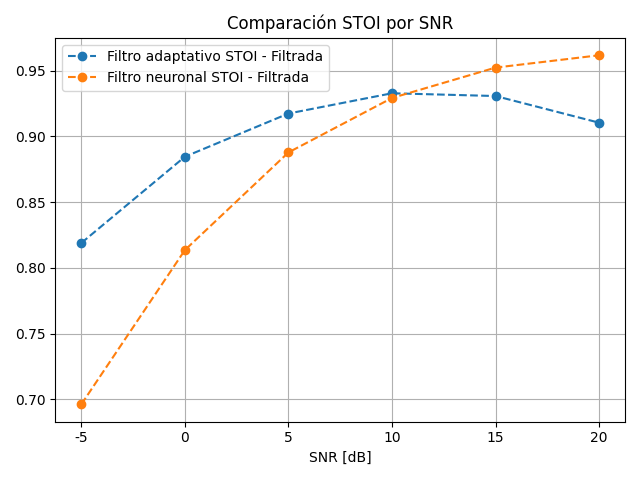
\includegraphics[scale=0.75]{images/ch8/comparison_stoi_by_snr.png}}
	\caption{Comparación STOI en función de la SNR.}
	\label{fig:ch8_stoi_comparison_by_snr}
\end{figure}

Para el caso de la STOI el filtro adaptativo fue superior hasta los $\SI{10}{dB}$, punto a partir del cual el filtro neuronal logró un mejor desempeño.  

Haciendo un análisis global respecto a PESQ y STOI se observa que el comportamiento del filtro neuronal es superior al adaptativo en bajos niveles de ruido (altos SNRs). Esto se debe a que el filtro neuronal logra un menor ECM que el adaptativo a medida que la SNR aumenta.

\begin{figure}
	\centering
	\centerline{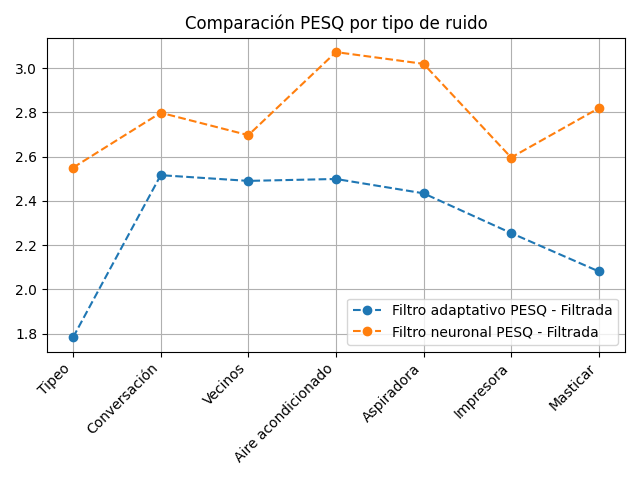
\includegraphics[scale=0.75]{images/ch8/comparison_pesq_by_noise_type.png}}
	\caption{Comparación PESQ en función del tipo de ruido.}
	\label{fig:ch8_pesq_comparison_by_noise_type}
\end{figure}

\begin{figure}
	\centering
	\centerline{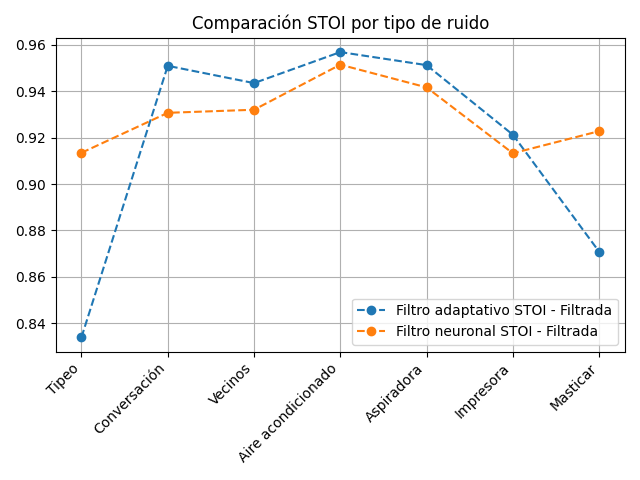
\includegraphics[scale=0.75]{images/ch8/comparison_stoi_by_noise_type.png}}
	\caption{Comparación STOI en función del tipo de ruido.}
	\label{fig:ch8_stoi_comparison_by_noise_type}
\end{figure}

También resulta interesante comparar como fue el desempeño de cada tipo de filtro en función del ruido, tanto para la medida PESQ como la medida STOI. En las figuras \ref{fig:ch8_pesq_comparison_by_noise_type} y \ref{fig:ch8_stoi_comparison_by_noise_type} podemos ver los resultados obtenidos.

En relación a la medida PESQ, se observa en la figura \ref{fig:ch8_pesq_comparison_by_noise_type}, que el filtro neuronal
fue superior en todas las clases de ruido. Este comportamiento va en linea con lo observado en la figura \ref{fig:ch8_pesq_comparison_by_snr} donde vimos que el filtro neuronal, en promedio, fue superior al adaptativo.


Para el caso de la STOI se observa un comportamiento esperado a partir del análisis de la figura \ref{fig:ch8_stoi_comparison_by_snr}, donde vimos que en promedio, el desempeño del filtro adaptativo fue superior. A excepción de los tipos de ruidos \emph{Tipeo} y \emph{Masticar}, el filtro adaptativo logro un mejor desempeño que el neuronal en termino de la inteligibilidad.